This chapter presents the results of applying our method to a selection of RSS feeds spanning various news categories from well known news;
\begin{itemize}[noitemsep]
	\item \textbf{Politics} from \textit{BBC News}, where we attempt to determine whether the map provides good coverage of the day's main stories (Section \ref{sec:politics}).
	\item \textbf{Business} from \textit{The Telegraph}, where we discuss best and worst case map layouts including common pitfalls (Section \ref{sec:business});
	\item \textbf{Sport} from \textit{The Guardian}, where we provide a warning on the risks of misinterpretation and false inferences (Section \ref{sec:sport}).
\end{itemize}

\section{UK Politics (BBC News) \label{sec:politics}}

The main topic threads for March 16\textsuperscript{th} 2017 in British politics were Scottish First Minister Nicola Sturgeon's call for a second independence referendum, the government's U-turn on National Insurance increases for the self-employed in the Spring Budget, and The Queen granting Article 50 royal assent, therefore enabling Brexit negotiations to begin.
\begin{figure}[htbp!]
	\centering
	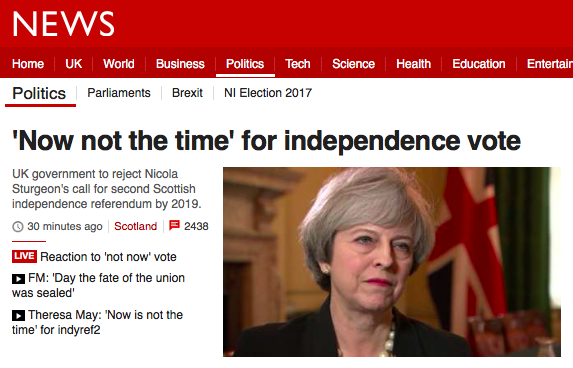
\includegraphics[width=.75\textwidth]{img/results/bbc-politics-frontpage.png}
	\caption{The front page BBC Politics article; drawn as (a) in Figure \ref{fig:bbc-pol}.}
	\label{fig:bbc-pol-home}
\end{figure}

To determine whether the map captured day's important political issues, we turn back to the native representation of the news. The BBC selected a piece on the proposed Scottish referendum as the front page article for their Politics page (Figure \ref{fig:bbc-pol-home}); a position which is generally indicative of importance.

In contrast, RSS feeds have no notion of relative content importance, so the system has no way of knowing this article should be included. Nevertheless however, when the article is parsed, its keyword vector contains \texttt{\{`Scotland': 1.09861\}} as the top entity. This term-frequency was strengthened by the transformation of every instance of the denominal adjective \textit{Scottish} into the noun form, \textit{Scotland}. The concentration of articles which focus heavily on Scotland (its coverage score of 182.644 was the third highest of the corpus) means it is selected as a metro line, resulting in the article being added to the map as we had hoped (see Figure \ref{fig:bbc-pol}).
\begin{figure}[htbp!]
	\centering
	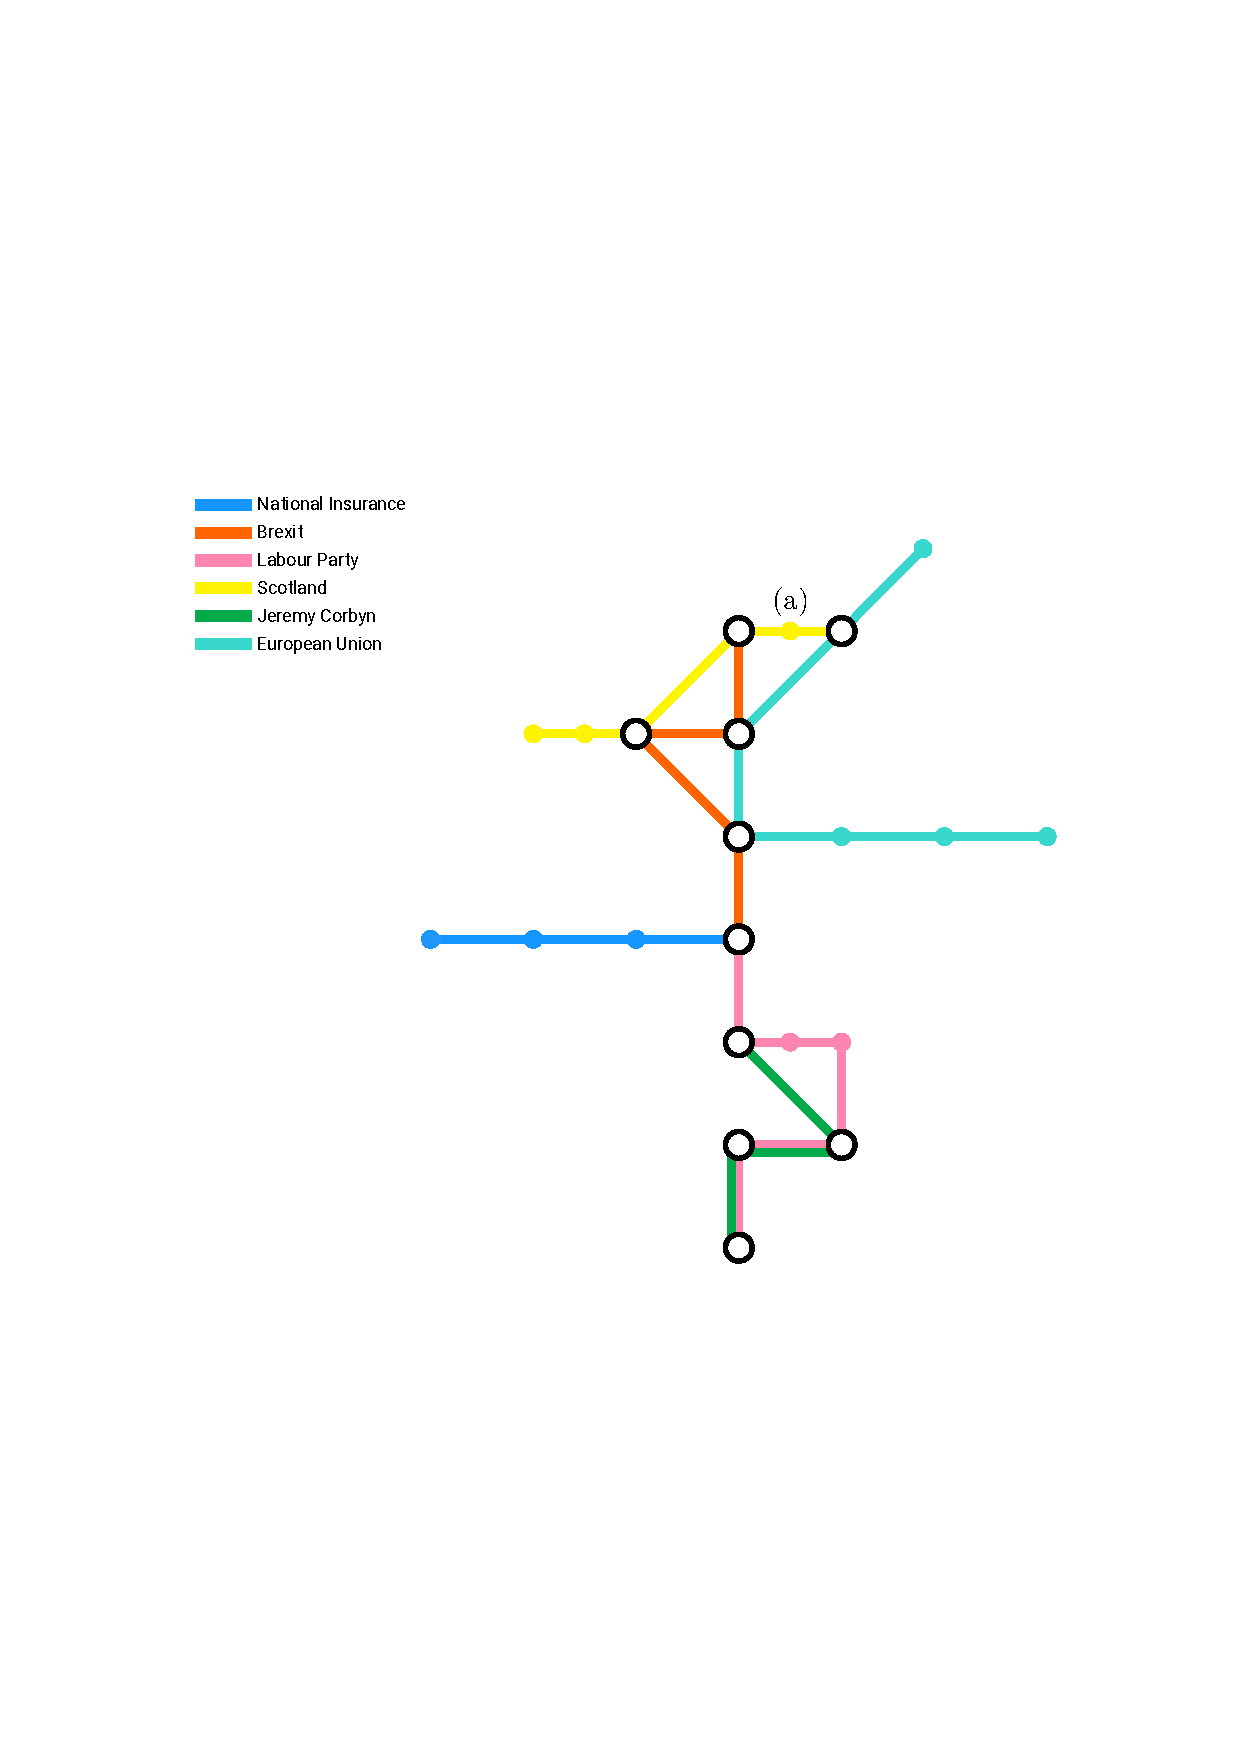
\includegraphics[width=.9\textwidth]{img/results/bbc-politics.pdf}
	\caption{A metro map covering the BBC UK Politics RSS feed (March 16\textsuperscript{th} 2017)}
	\label{fig:bbc-pol}
\end{figure}

As well as a series of articles following the progression of the proposed referendum, the system also selects the other two main threads as metro lines. \textit{National insurance} is selected despite its relatively short length due to its low affinity with the other lines. The system interprets this low affinity as the line covering a set of articles which no other line has, which boosts its likelihood of selection.

Despite being entirely subsumed by the \textit{Labour Party} line, \textit{Jeremy Corbyn} is still selected for the map because of the strength of its keyword score within the articles which contained it. Intuitively, we would hope that users realise lines which are entirely subsumed by other lines are important in their own right, while still being closely related to their subsuming entity.

\section{Business (The Telegraph) \label{sec:business}}

The system also performs well for international business news, where entities are typically the names of companies and organisations as opposed to people. NLTK Struggles with place names which have containment issues, for example, `City of London' is split into \textit{City} and \textit{London}, and `Bank of England' into \textit{Bank} and \textit{England}. \textit{London} and \textit{England} are then penalised by tf-idf for being common, but  \textit{Bank} and \textit{City} are both selected as metro lines. In spite of this contrived error, the map is still largely usable and exhibits good coverage.
\begin{figure}[htbp!]
	\centering
	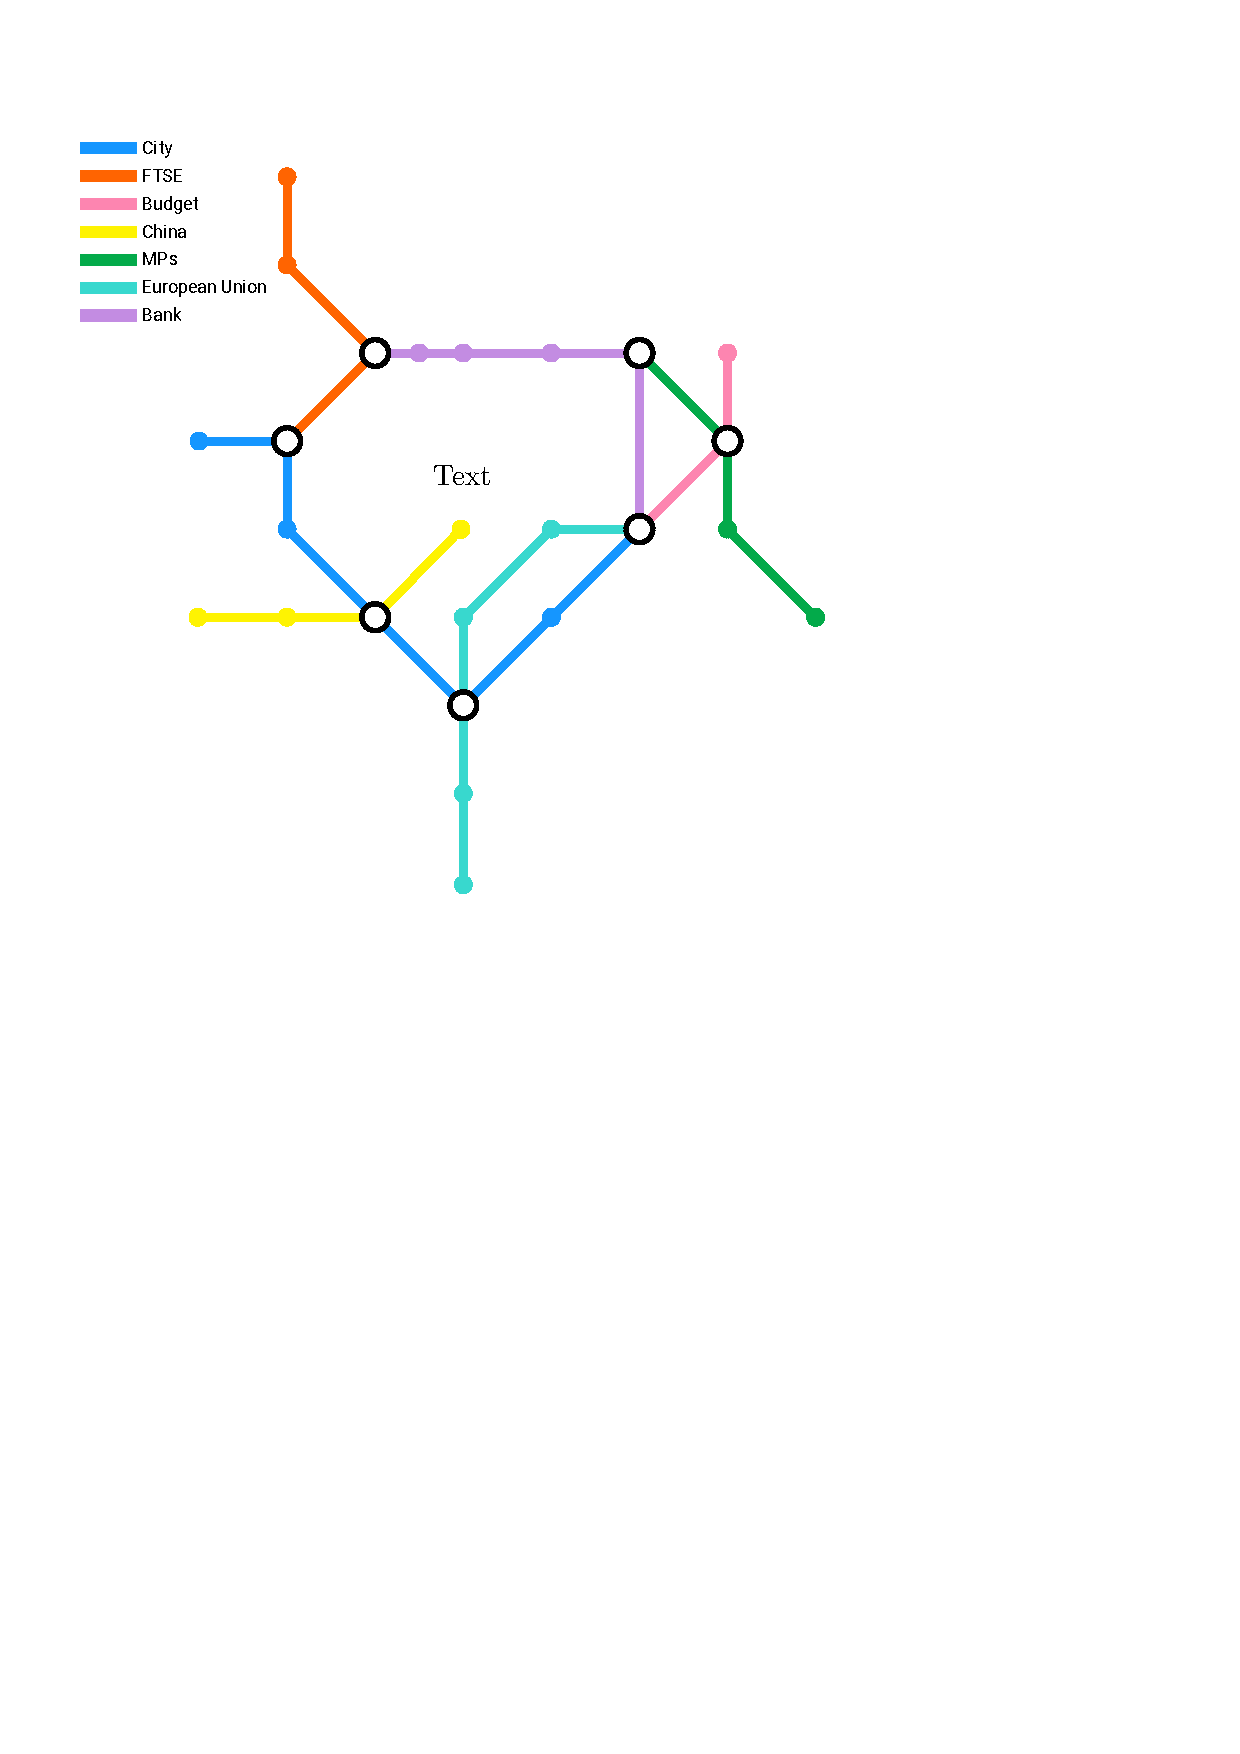
\includegraphics[width=.9\textwidth]{img/results/telegraph-business-tfidf.pdf}
	\caption{A metro map covering The Telegraph's Business RSS feed (March 17\textsuperscript{th} 2017)}
	\label{fig:telegraph-business}
\end{figure}

From an aesthetic perspective, a common pitfall of our approach is visible on the \textit{Bank} line (Figure \ref{fig:telegraph-business}). During repeated passes along each octilinear line, stations are moved to the midpoint of their immediately adjacent neighbours, which results in noticeably variable edge lengths. A fix for this would be to iterate between pairs of stations which represent the endpoints of a run of stations all with weight two and distribute the accumulated stations at uniform intervals between the two points (Figure \ref{fig:equal-spacing}).
\begin{figure}[htbp!]
	\centering
	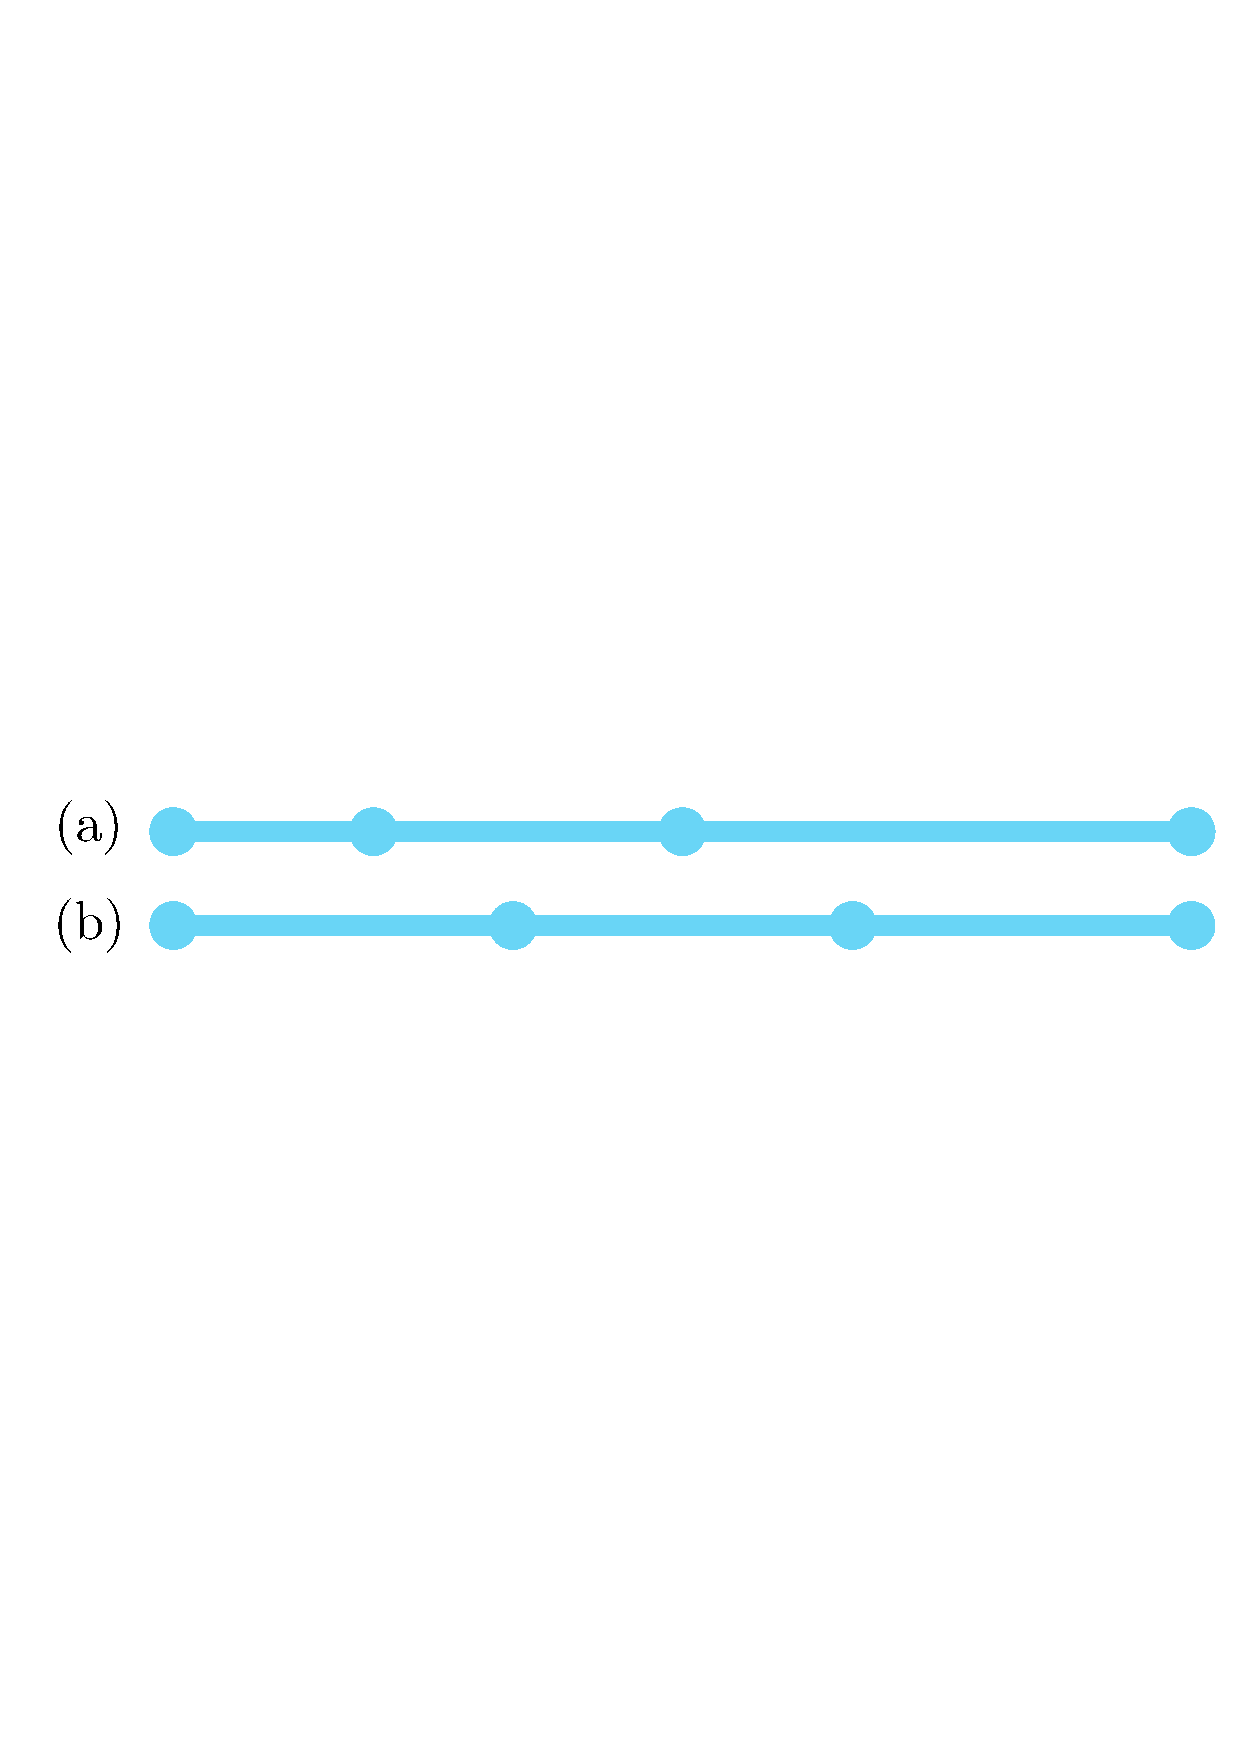
\includegraphics[width=.5\textwidth]{img/results/equal-spacing.pdf}
	\caption{The redistribution of unbalanced edges along a line}
	\label{fig:equal-spacing}
\end{figure}

A second pitfall is the inability of the algorithm to smooth the \textit{European Union} line in Figure \ref{fig:telegraph-business-poor} between two points which are not octilinear to each other. The shape of the \textit{China} line here is also frequently observed, because the initial force-directed algorithm causes lines to form circular arrangements, which are then snapped to co-ordinates which form squares.
\begin{figure}[htbp!]
	\centering
	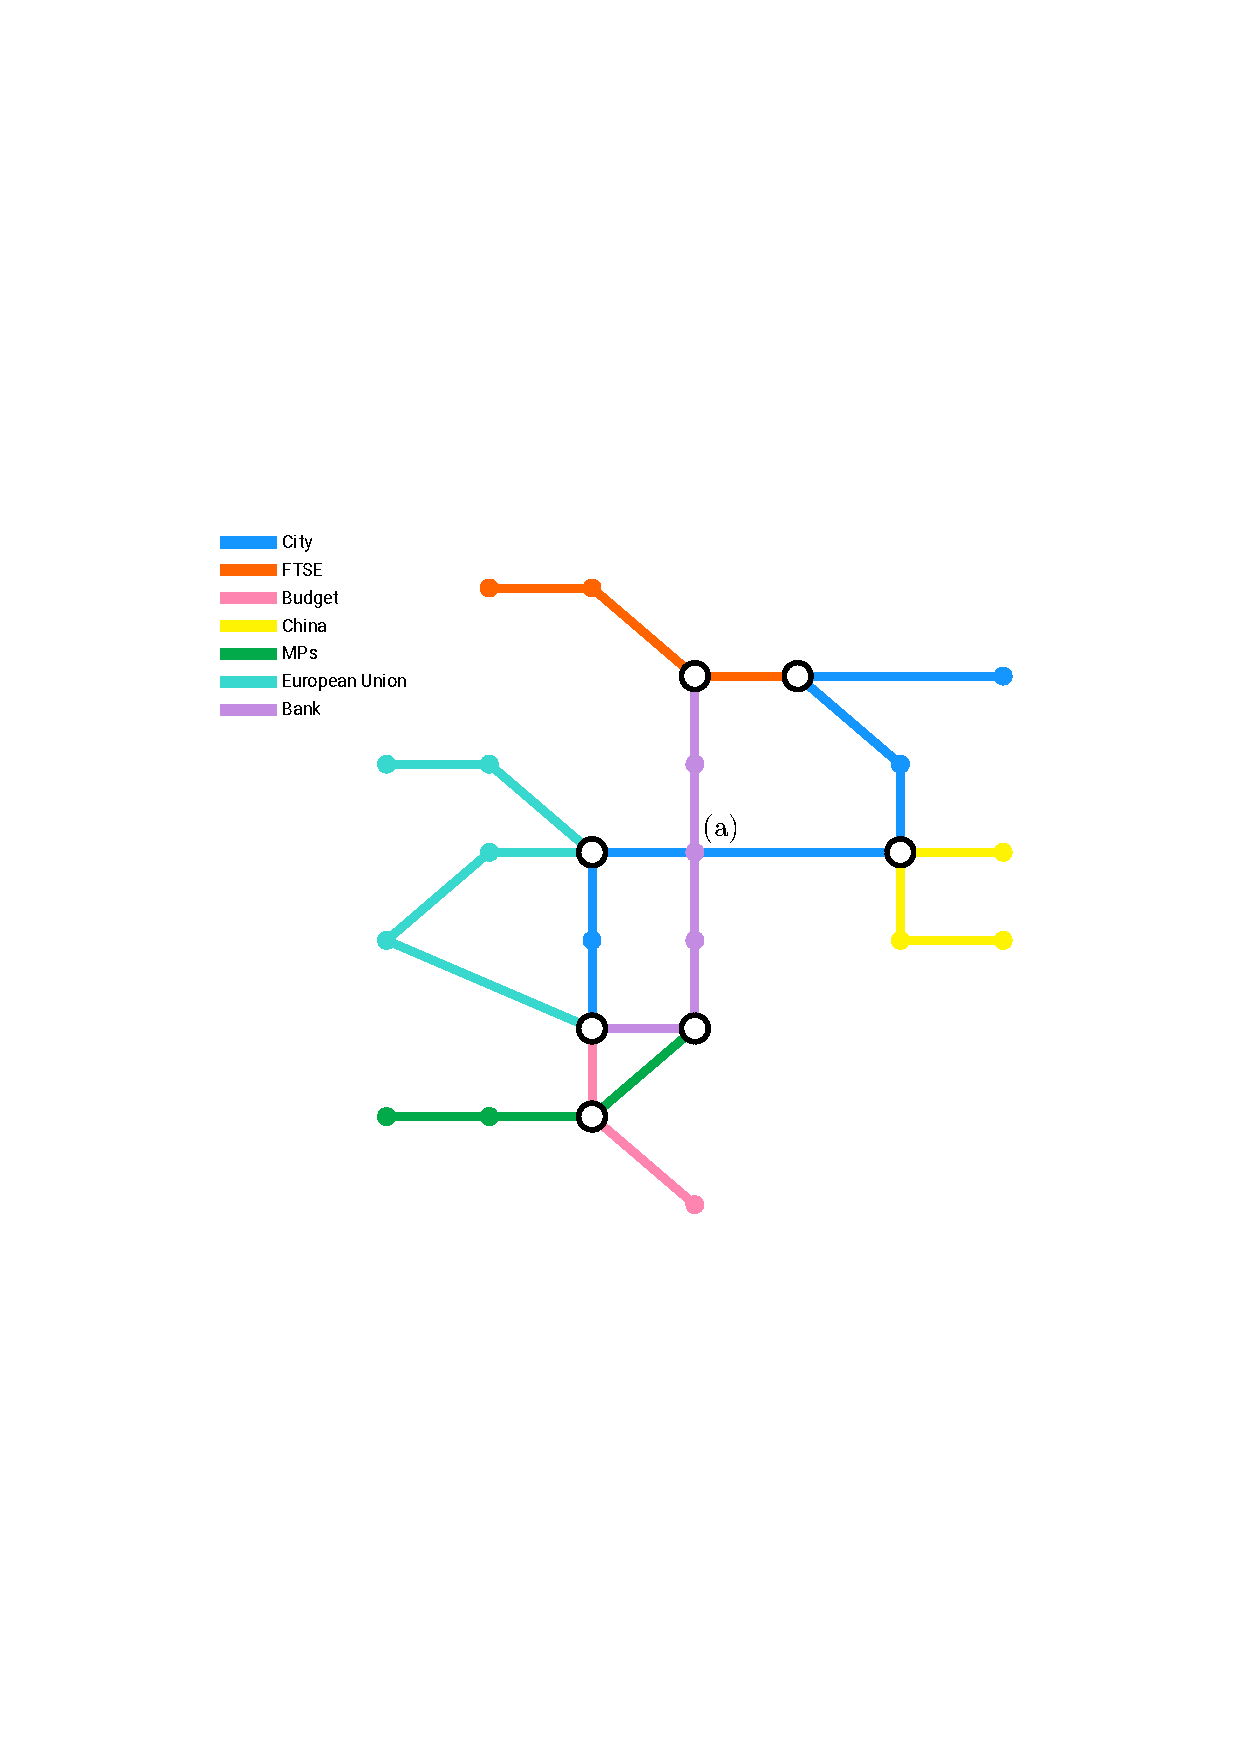
\includegraphics[width=.8\textwidth]{img/results/telegraph-business-poor.pdf}
	\caption{A poor embedding of the map in Figure \ref{fig:telegraph-business}}
	\label{fig:telegraph-business-poor}
\end{figure}


\section{Sport (The Guardian) \label{sec:sport}}

Sports journalism was popular among the participants of the Associated Press [\citeyear{anewmodelfornews}] study, in part because of the clean cut categorisation of teams within sports, within countries where applicable. Story resolution could be always achieved on a match-by-match basis, or over one or more seasons of predefined length. Current events journalism, in contrast, includes stories which are complex and sprawling in nature, often continuing over a period of days, weeks or even years.

Our system was designed for use with current events articles rather than sports content, but the results obtained through doing so bring to light some interesting issues which were not evident in previous examples, and therefore warrant discussion.
\begin{figure}[htbp!]
	\centering
	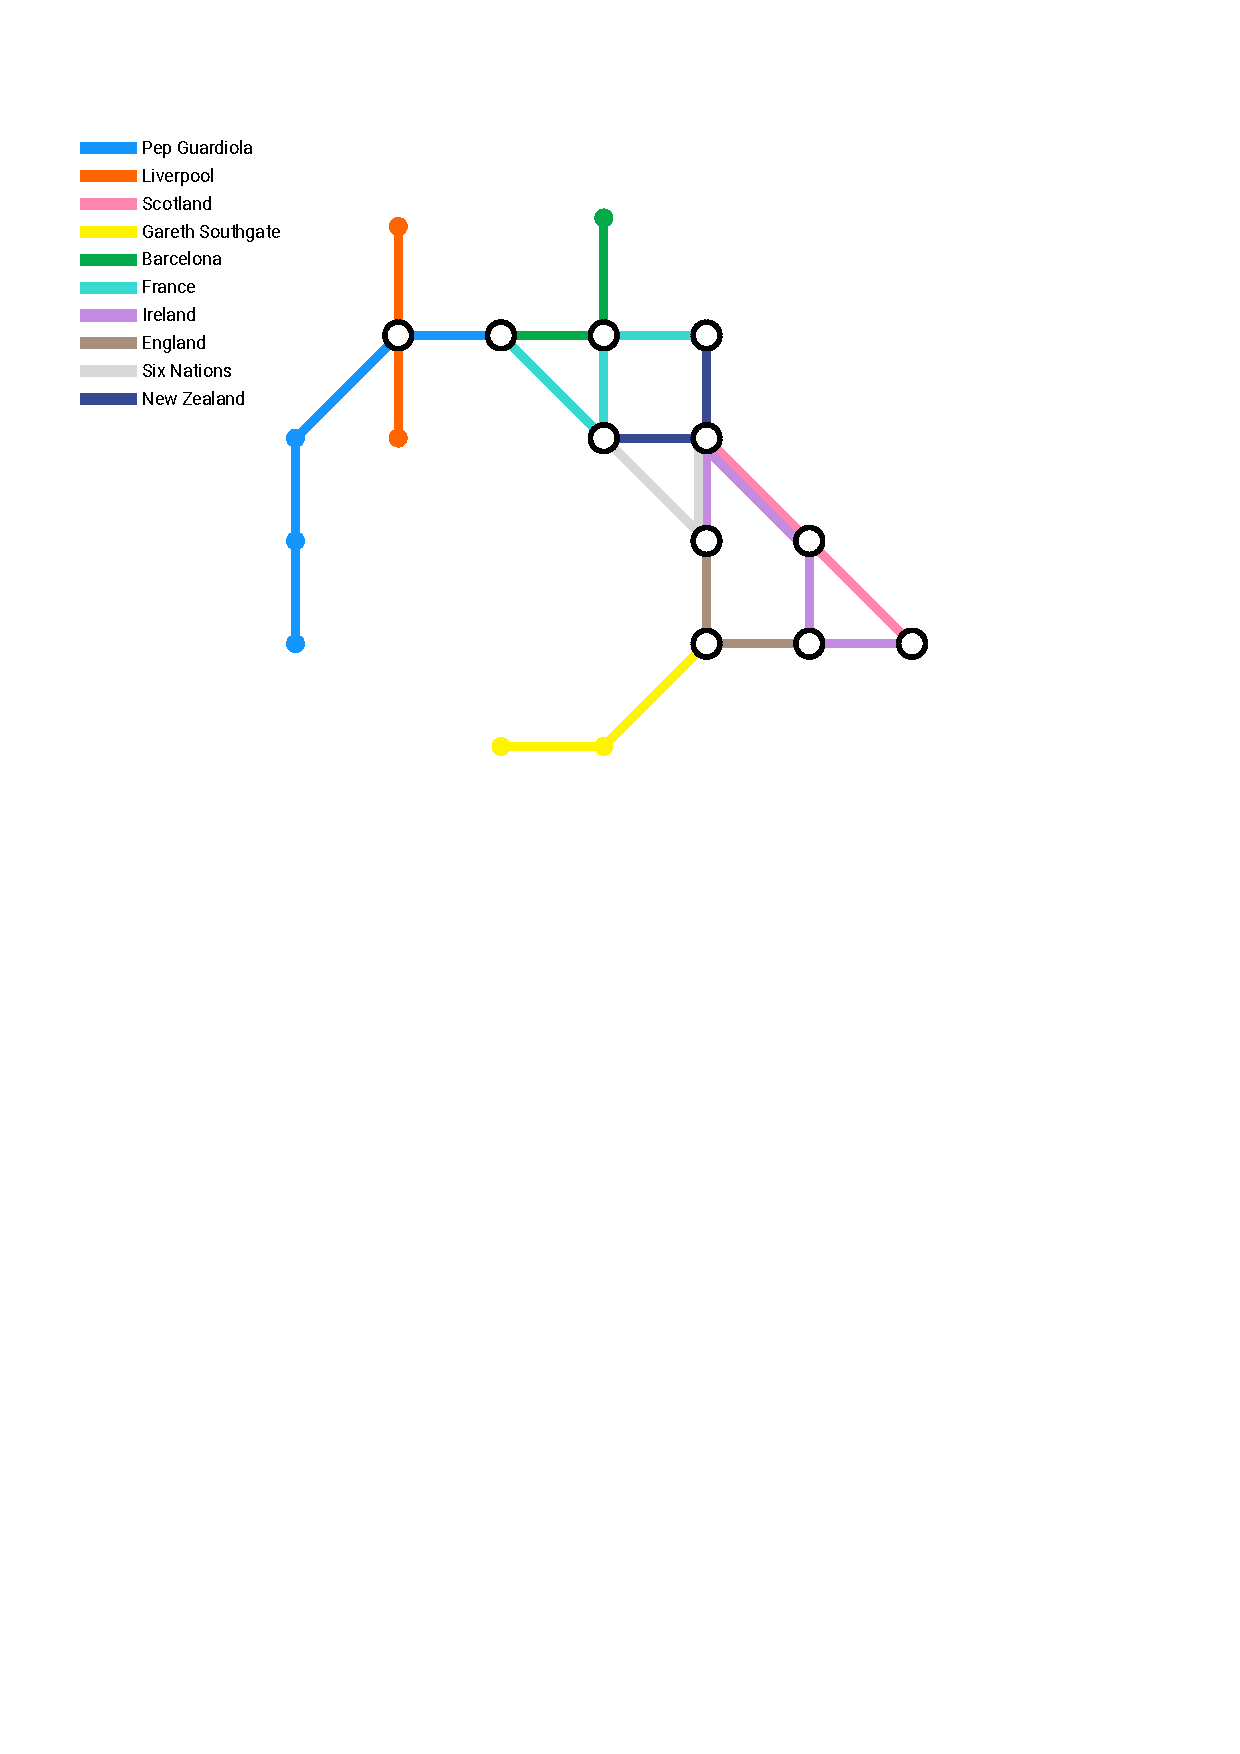
\includegraphics[width=\textwidth]{img/results/guardian-sport.pdf}
	\caption{A metro map covering the Guardian Sport RSS feed (March 16\textsuperscript{th} 2017)}
	\label{fig:guardian-sport}
\end{figure}

If someone who knew very little about rugby were to look at the metro map on sports and see \textit{Six Nations}, they would most likely (and correctly) assume that it is the name of a tournament with six participating countries. Using only the connections drawn on the map however, they may also assume that all five countries whose metro lines intersect with Six Nations are participants. This is incorrect; New Zealand, which intersects twice, is not.

This is a good example of a metro map which exhibits desirable aesthetic properties and good coverage, but which is ambiguous and therefore uninformative at a thematic level. The names of the majority of the metro lines are countries, which create widespread entity ambiguity problems; does \textit{England} imply the football team or the rugby team? The answer to this question is unfortunately both, as the system is unable to disambiguate. The risk of misinterpretation by a user leading to confusion and contributing further to information overload is of course ever present, but particularly noticeable in this example.

The quality of the metro lines on this map confirmed our suspicious that the system is not practical for use with corpora which contain a large number of ambiguous entities. That is not to say, however, that metro maps are inappropriate for all news feeds related to sport. Generating a metro map based on The Guardian's Football RSS feed (Figure \ref{fig:guardian-football}) does not lead to the same team name ambiguities, and therefore results in an unequivocally distinct set of metro lines.\\

\begin{figure}[htbp!]
	\centering
	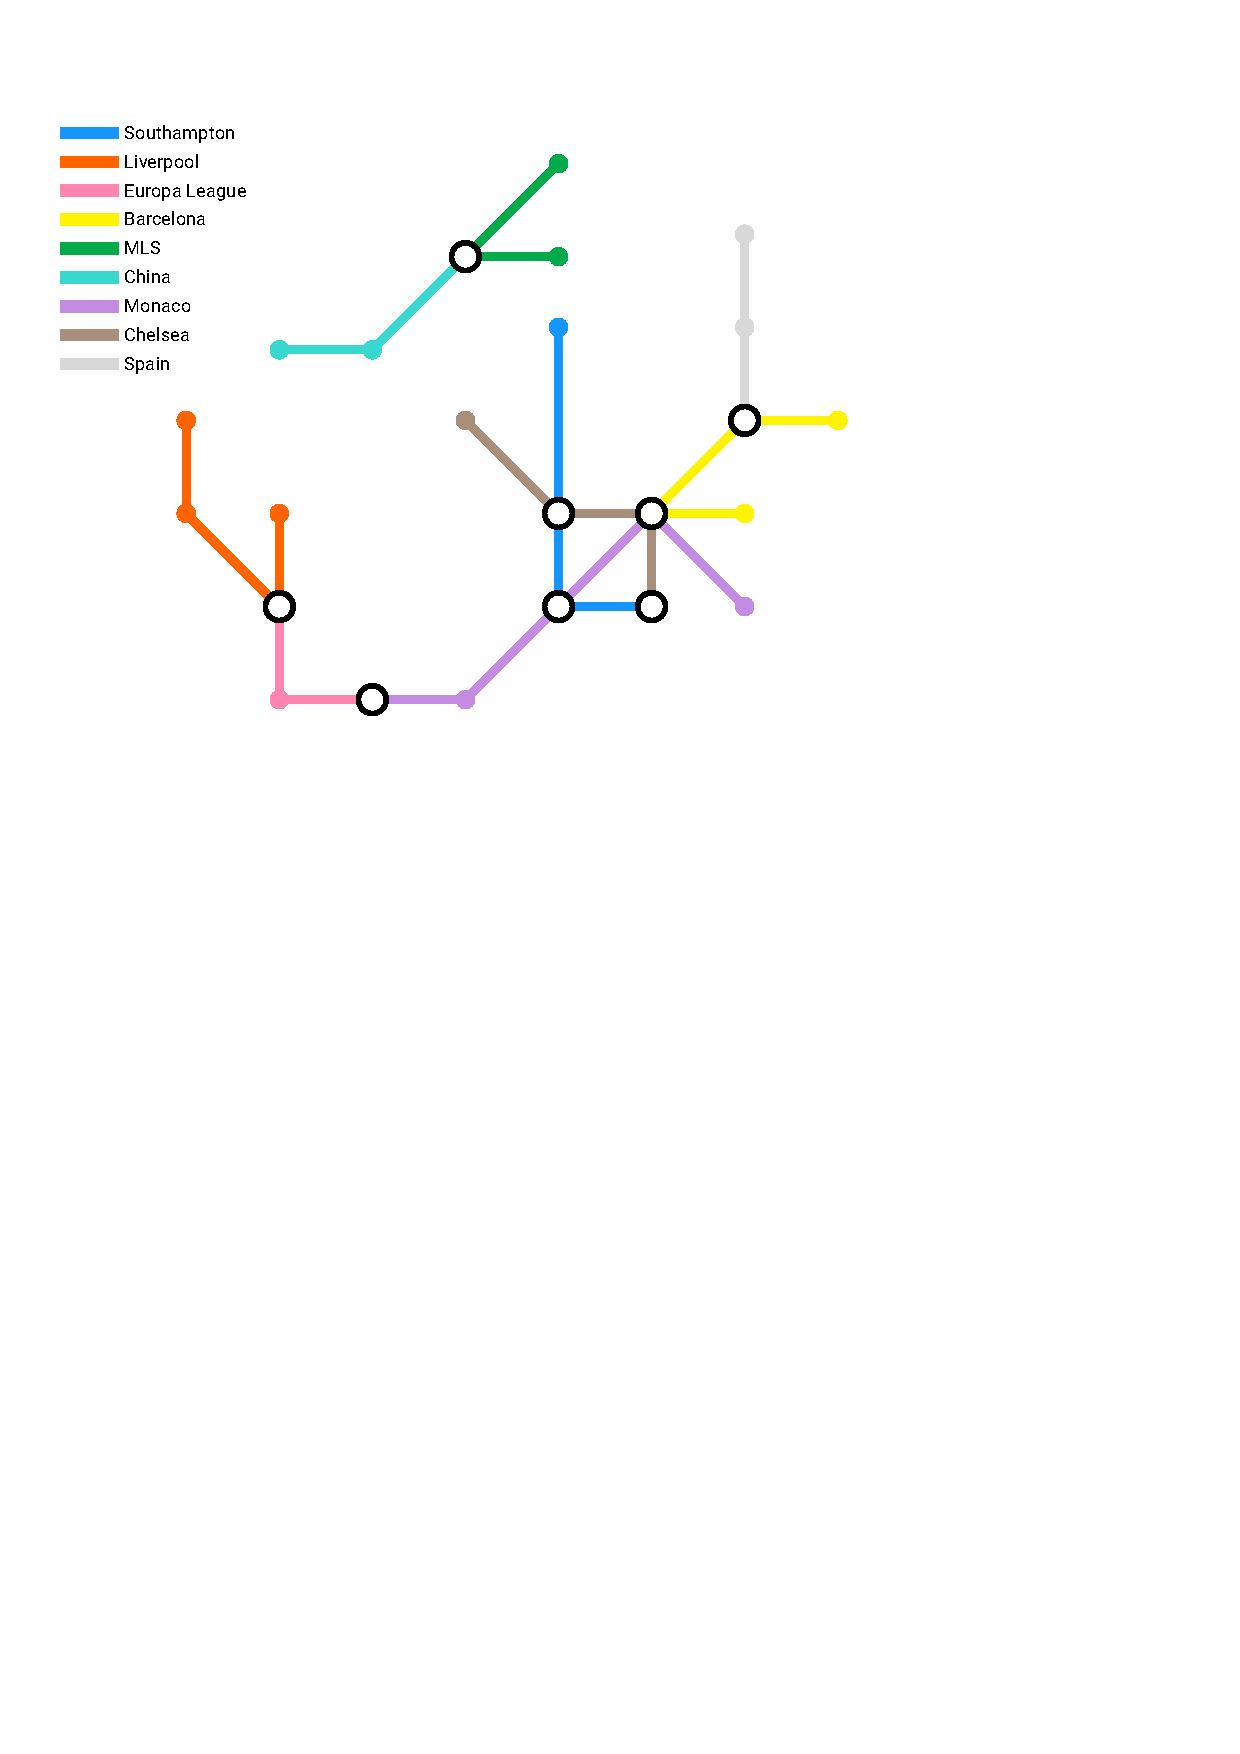
\includegraphics[width=\textwidth]{img/results/guardian-football.pdf}
	\caption{A metro map covering the Guardian Football RSS feed (March 17\textsuperscript{th} 2017)}
	\label{fig:guardian-football}
\end{figure}

News coverage for individual sports and leagues, it transpires, can be well represented on metro maps. This is mainly due to keyword extraction being less complex in this domain; the names of most teams and sports personalities are easily identifiable with a knowledge base. To only select \textit{teams} as metro lines, we could simply filter out other entities at the Knowledge Graph stage, using the \texttt{Thing > Organization > SportsOrganization > SportsTeam} type from Schema.org. The same principle could be applied to countries or athletes, in order for users to adjust the schema represented by the metro lines at a \textit{zoom-and-filter} level \citep{TheEyesHaveIt}.

Generalising this relationship between well defined schemas and a well defined set of metro lines to domains other than sports would suggest that in order to improve line selection for any map, it may be beneficial to restrict line choice to those which fit certain predefined types, such as \texttt{Thing > Person}, \texttt{Thing > Organization}, and \texttt{Thing > Place}. This kind of schematisation immediately leads to the question of which entities we should consider useful. The answer to this question may be domain-specific, user-specific, or most likely a combination of the two.

\section{Summary}

This chapter presented three different perspectives from which the results of the system can be analysed; by content, by layout, and by context. 

Firstly, we verified that our maps provide sufficient coverage of topics which were deemed significant by the original news source, and discussed a concrete example of two topics being selected as metro lines despite their high affinity with each other.

Following on from content, we took a step back and evaluated the maps purely in terms of the success of their embeddings. Best and worst case layout examples were provided examples for a particular current events map, where we identified common weaknesses of the map layout algorithm, in particular the inability of the layout algorithm to smooth non-octilinear edges once stations have been marked as placed.

Finally, we used the system to generated a metro map for a corpus it was not designed to be used on; international sports news. This demonstrated the need for common entities within a corpus to be identifiable without ambiguity, unlike for instance the names of international sports teams between different sporting disciplines. We did however find that the system generates useful maps for sports news corpora when restricted to individual sports, where there is less obvious name ambiguity, and the corpus itself suggests a schema for expected entities.

Section \ref{sec:sport} ended with a more general note on the utility of a schema during the graph formation process, where metro lines are chosen from a pool of candidate keywords. Being able to select or reject lines based on a schematisation of expected entities within a corpus was not something we had considered during the implementation of the system, as it only came to light by using the system on data it was not designed for. Nevertheless, schema-based metro line selection and pruning is a novel concept which merits further investigation in future systems.

While accurate topic coverage and octilinear embeddings may be sufficient to evaluate the keyword extraction and map layout processes respectively, they do not provide any real insight into usability. That is to say, we may have designed a system which generates \textit{good} metro maps both contextually and aesthetically, but the maps themselves have not been shown to have any effect on information overload. The next chapter therefore presents this evaluation in the form of two experiments.

